\documentclass{sig-alternate}

\usepackage{epsfig}
\usepackage{subfigure}

\makeatletter
\def\@copyrightspace{\relax}
\makeatother

\title{Efficiency Simulation for Bus Traffic in Taipei City}
\numberofauthors{3}
\author{
 \alignauthor
 Tsung-Hsien Wen\\
 	\email{r00921033@ntu.edu.tw}
 \alignauthor
 Po-Chun Hsu\\
 	\email{r00921034@ntu.edu.tw}
 \alignauthor
 Heng Wang\\
 	\email{r00944042@ntu.edu.tw}
 }
\begin{document}
\maketitle

\begin{abstract}
For newcomers in Taipei, the bus system there is hard to figure out since there are too many bus lines.
In addition, some of the lines are tortuous and make travellers spend much more time than expected.
Consequently, travelling by bus might be inefficient for those who are not experienced in taking bus in Taipei.
From another perspective, this kind of bus network is energy-consuming as well.
A chessboard-like bus network has been thought to be a solution to these problems for many years, although it has not been promoted successfully in Taipei.
We thus want to know whether a chessboard-like bus network works better in Taipei.
We set up a simulation to observe what are the pros and cons of a chessboard-like bus network and the current bus network.
We encoded a part of roads in Taipei into a graph.
Two types of agents, buses and clients, are placed in the simulation environment.
In order to simulate the behaviors of buses, we record the routes and intervals of buses from the Taipei e-bus website.
We also set up different scenario types to simulate client behaviors at different time points of a day.
The simulation results suggest that a chessboard-like bus network is more efficient in terms of the resource utilization.
Even though the data are still limited so real-world clients is hard to model, this simulation is an initial attempt to model the bus activities in Taipei and gives us some insight on future policies of public transportation.
\end{abstract}

\section{Introduction}
In Taipei City, there are about 300 bus routes in operation, which makes the bus system is hard to figure out for those who are not familiar with taking bus here.
Due to the overfull bus routes, people living in Taipei City could have observed that many routes overlap with others and that sometimes bus jam occurs at a bus stop.
In addition, some of the bus routes are tortuous, so travellers on buses might spend more time than expected.
From the above problems, it can be speculated that the energy consumption of buses in Taipei City is unnecessarily high.
On the whole, bus transportation could be less efficient and more resource-consuming than other transportation.
These problems have existed and been noticed for many years.
Many people have tried to find out whether there exists a bus system working better in Taipei City.

A chessboard-like bus network has been thought to be a solution to the above problems.
In the late 1980s', an initial prototype of a chessboard-like bus network started to be operated, but the new routes were not used commonly then.
Most of the routes are therefore not in operation now.
Nevertheless, in 2006, the the Commissioner of the Taipei City Department of Transportation tried to promote a new bus route network again.
Due to opposition from some frequent bus takers who did not transfers between buses and, more importantly, from the bus companies which had vested interests (about 15 bus companies are in operation), the new policy was not executed.
In 2010, Taipei City councilors hurried the government to promote the policy, but it is still the old system operated in Taipei City.

Despite that the problems of bus transportation is not only a engineering problem, we want to know whether a chessboard-like bus network is more efficient or more convenient than the current system in Taipei City theoretically.
The purpose of this project is to set up a simulation of behaviors of buses and clients and to observe what influences the efficiency of the bus traffic system.

\section{Data collection}
For our real-case simulation, we transform a map of part of Taipei City into a graph with roads as edges and intersections as nodes.
We need distances between each two nodes, current traffic information, stops of the bus routes and time intervals of the buses.
They are all available but are hard to fetch automatically.
To get these data, we have used the most powerful parser in the world!
We collect the road conditions from Google Map and the bus information from the website of Taipei Public Transportation Office manually.

We select an area of Taipei City as in Figure~\ref{fig:tpemap}.
We transform it into a graph as in Figure~\ref{fig:graphex}, where edges represent the roads in the area and nodes represent the intersection of the roads.
On the graph, we add the information of roads as in Figures~\ref{fig:node} and~\ref{fig:edge}.
We record the bus routes and intervals as in Figures~\ref{fig:bus}.

\begin{figure}
\centering
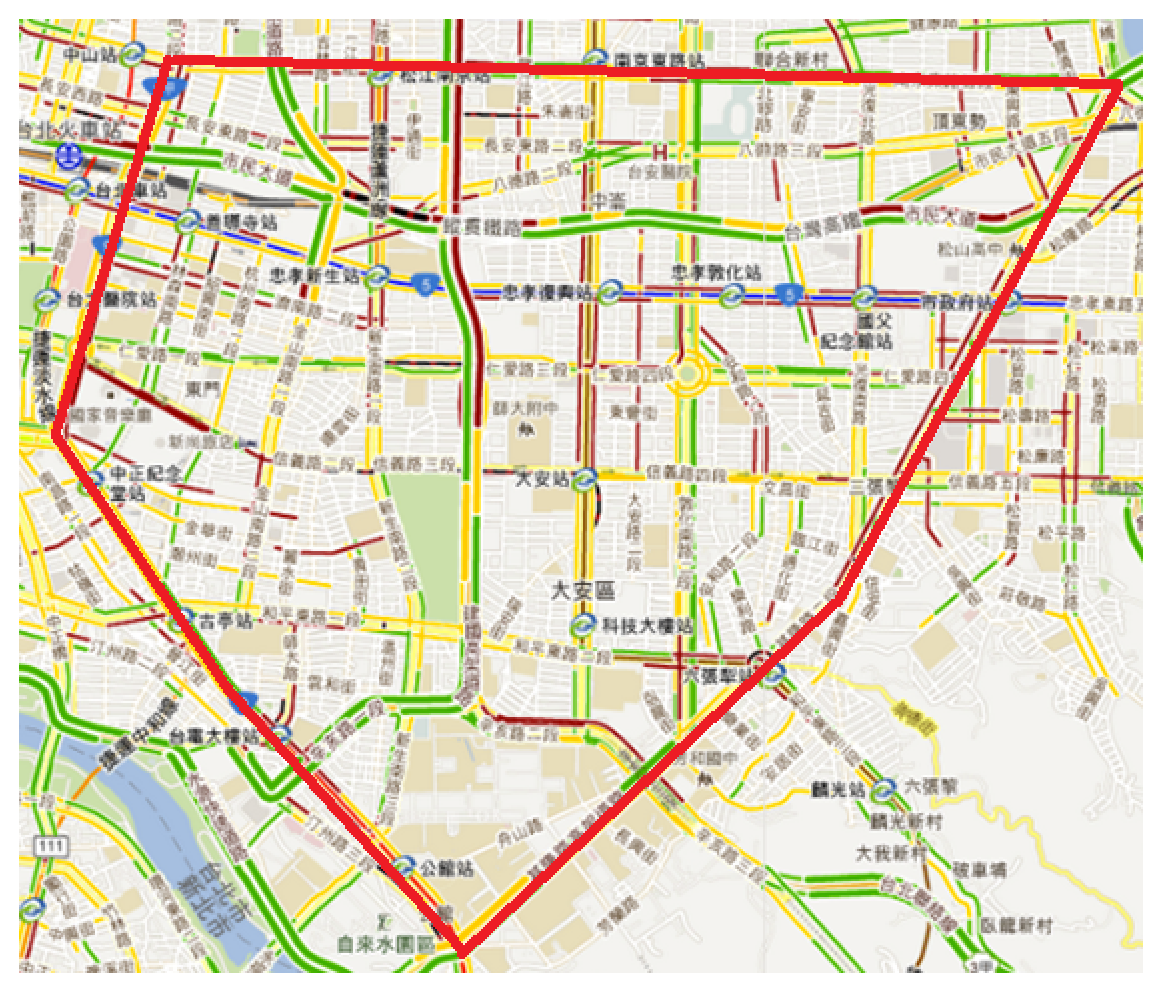
\includegraphics[height=2.5in, width=3.1in]{taipeimap.eps}
\caption{The framed area is transformed into the graph shown in Figure~\ref{fig:graphex}.}
\label{fig:tpemap}
\end{figure}

\begin{figure}
\centering
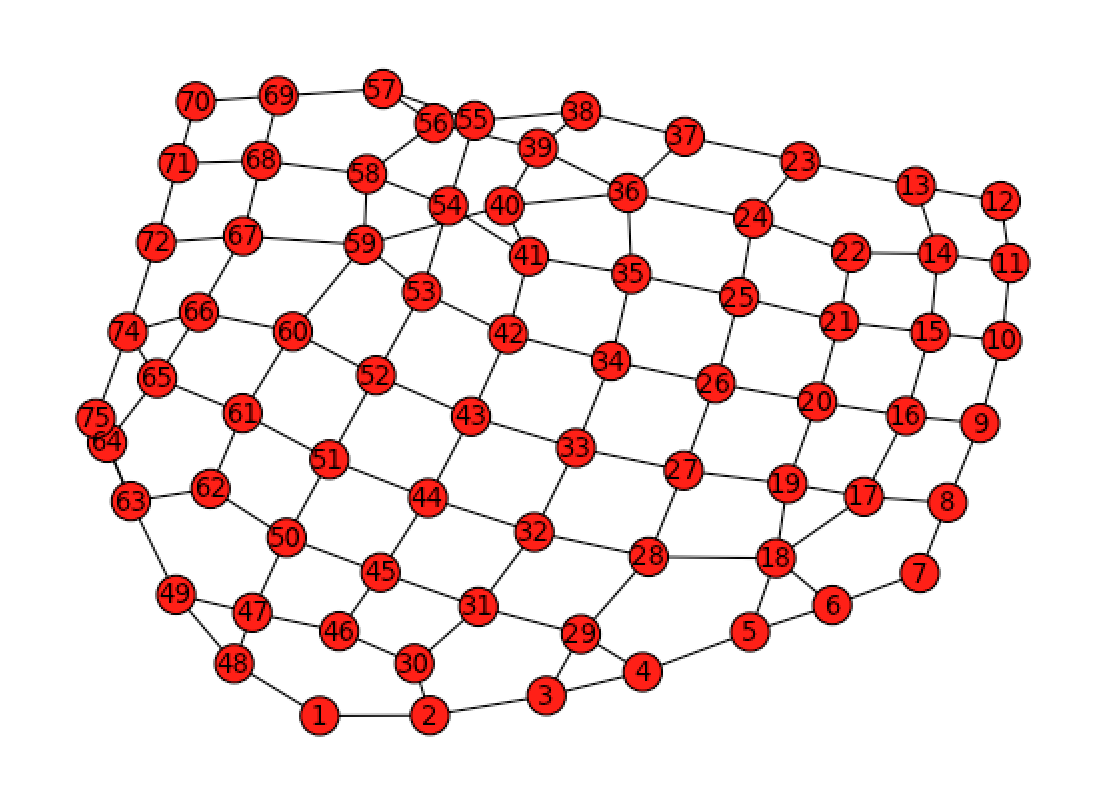
\includegraphics[height=2.2in, width=3.1in]{graphexample.eps}
\caption{In this graph, edges represent the roads and nodes represent the intersections.}
\label{fig:graphex}
\end{figure}

\begin{figure}
\centering
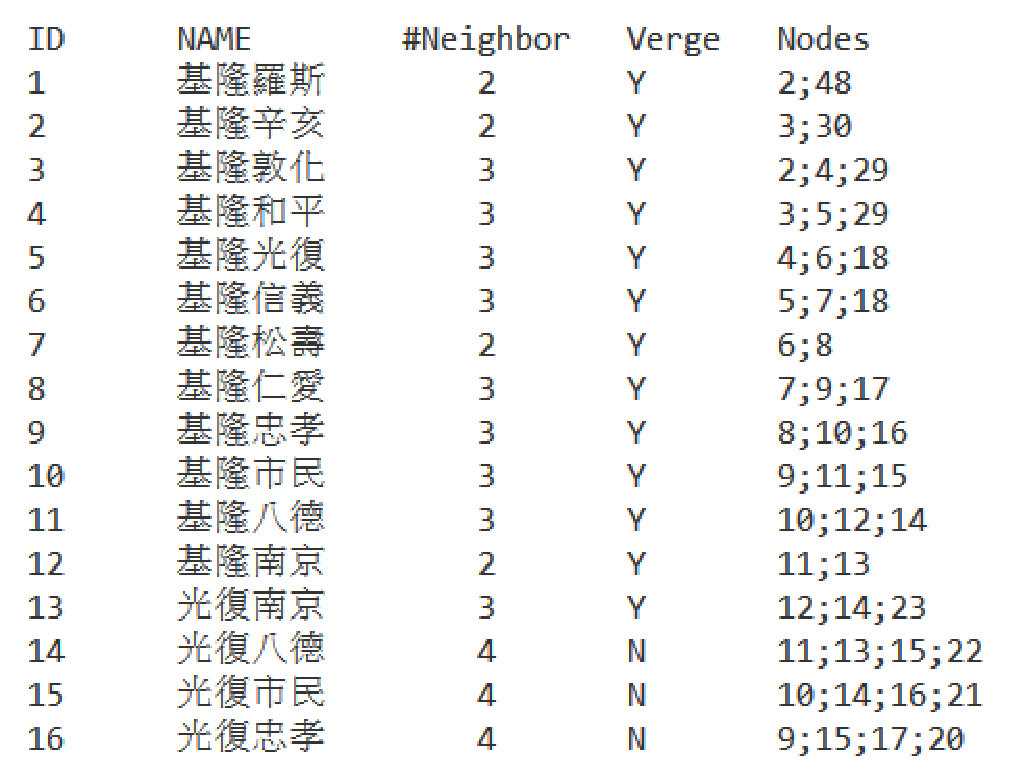
\includegraphics[height=2.4in, width=3.1in]{node.eps}
\caption{Part of the node information (totally 74 nodes). The entries for each node are its ID number, its name, its number of adjacent nodes, whether this node is on the verge, and its adjacent nodes.}
\label{fig:node}
\end{figure}

\begin{figure}
\centering
\subfigure[]{
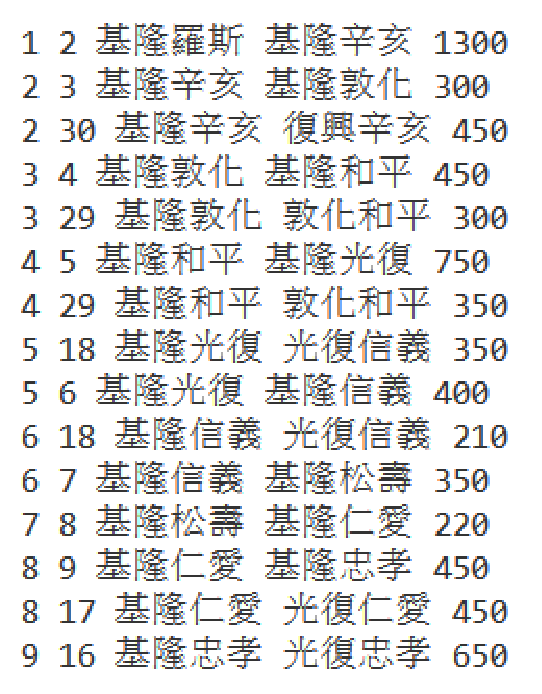
\includegraphics[height=1.5in, width=1.2in]{edge.eps}
\label{subfig:edge}
}
\subfigure[]{
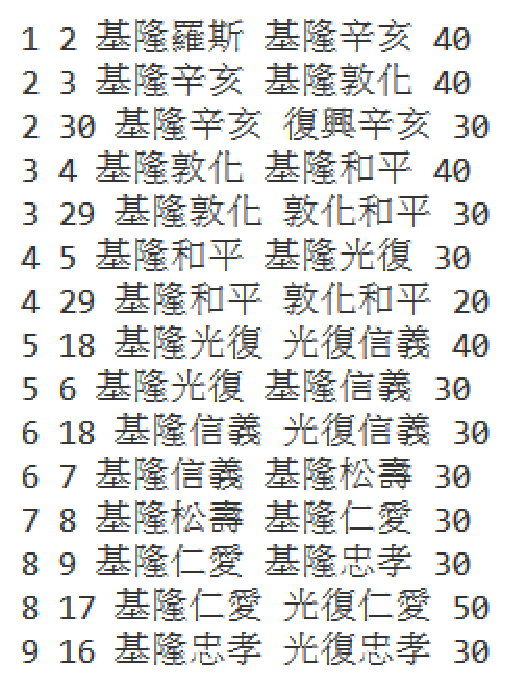
\includegraphics[height=1.5in, width=1.2in]{traffic.eps}
\label{subfig:traffic}
}
\caption{Figure~\ref{subfig:edge} is part of the edge information (totally 134 edges), where the entries for each edge are its two ends, the two ends' names, and the distance between the two ends; Figure~\ref{subfig:traffic} is part of the traffic conditions, where the
number in the last entry is the speed buses can drive at on the corresponding edge.}
\label{fig:edge}
\end{figure}

\begin{figure}
\centering
\subfigure[]{
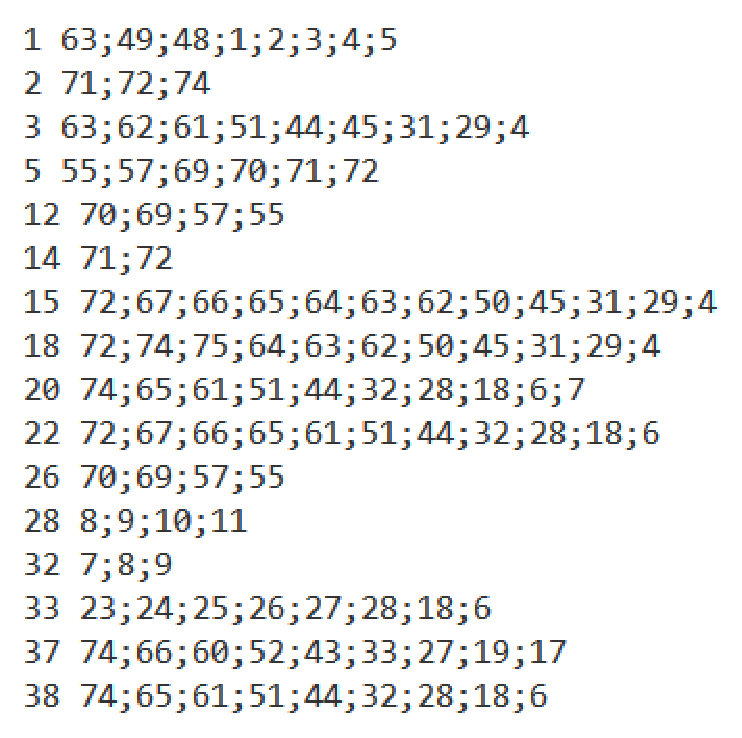
\includegraphics[height=1.6in, width=1.5in]{bus.eps}
\label{subfig:route}
}
\subfigure[]{
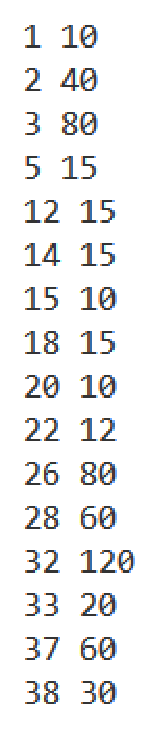
\includegraphics[height=1.6in, width=0.3in]{interval.eps}
\label{subfig:interval}
}
\caption{Figure~\ref{subfig:route} is part of the bus route information (totally 124 routes), where the entries for each bus are its route number and the stops (in the selected area) on its route; Figure~\ref{subfig:interval} is part of the bus interval information, where the
number in the second entry is the departure interval of the corresponding route.}
\label{fig:bus}
\end{figure}

\section{Agents}
\subsection{Buses}
\subsection{Clients}
Client agents are generated on nodes with a randomly chosen destination.
The number of clients generated depends on the type of scenario.
In the next section, we have a more detailed explanation about this.

In order to reduce the computational cost, we use a simple greedy algorithm to model the behavior of a client.
If a client is at a bus stop, it first compares all the buses stopping at this bus stop.
The client choose a bus the next stop of which is the closest to the destination.
If this bus can take it to a node which is closer to its destination than its current location, it gets on this chosen bus.
Otherwise, the client wait for another minute at the stop.
Indeed, it is not intuitive for us.
This modelling method has much room for improvement.

\section{Simulation}
In this section, we first introduce the environment settings of our simulation.
Three scenarios and different policies of bus agents are taken into consideration.
After that, we present the experimental results of the different environment settings.

\subsection{Environment Settings}
In our simulations, we set one minute as the basic unit of time.
The virtual buses and clients take actions at every minute.
We run 10000 units of time for each type of settings to get stable results.

We use three types of scenarios --- off-peak time, morning rush hours and evening rush hours.
For instance, during the morning rush hours, many clients could travel from the suburb to downtown Taipei.
That is, a client is more possible to move from the nodes on the verge of the selected area to the node inside the area.
Therefore, we set the three scenarios in the following way.
In the off-peak scenario, we generate clients form every node at every minute.
The number of clients to generate is sampled from a Gaussian distribution with a mean of 1.2 and a standard deviation of 0.5.
In the morning-rush-hour scenario, the number of clients to generate at the side nodes is increased --- sampled from from a Gaussian distribution with a mean of 3.6 and a standard deviation of 0.5.
In the evening-rush-hour scenario, this modification is operated on the inner nodes.
Once a client is generated, it randomly choose another node as its destination.

\subsection{Policies of Bus Agents}
\subsection{Results}

\section{Conclusion}

\end{document}